% Quelle: https://tex.stackexchange.com/questions/512240/3d-bang-boom-shape-in-tikz

\documentclass{article}

\usepackage[table,xcdraw]{xcolor}
\usepackage[utf8]{inputenc}
\usepackage{tikz}
\usetikzlibrary{shapes,snakes}
\usetikzlibrary{arrows.meta}
\usetikzlibrary{calc,patterns,angles,quotes}
\begin{document}
\begin{figure} 
\centering
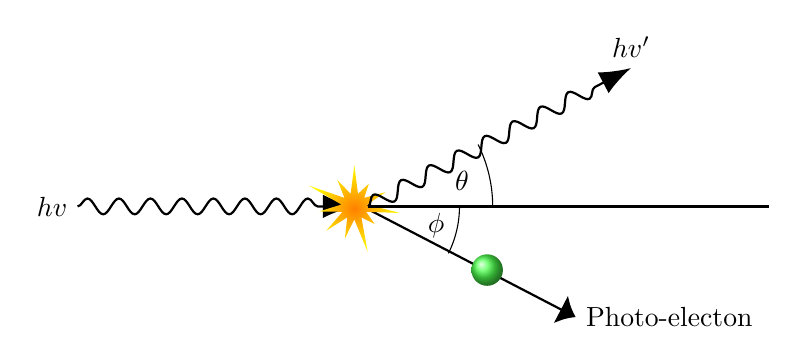
\begin{tikzpicture}
\draw [black, thick ,-{Latex[length=4mm]},decorate, decoration={snake,amplitude=1mm,segment length=4mm,post length=4mm}, label=left:Incident photon] (-100pt,0pt) node[left]{$hv$} -- (0,0pt);
\draw [black, thick ,-{Latex[width=4mm, length=6]}] (3pt,0pt) -- (80pt,-40pt) node[right]{Photo-electon} coordinate (d);
\node[starburst,inner color=orange,outer color=yellow,starburst points=11] at (0,0pt) {} coordinate (b);
\shade[ball color=green!70!white] (48pt, -23pt) circle (.2cm);
\draw [thick] (5pt,0pt) -- (150pt,0pt) coordinate (a);
\draw [black, thick ,-{Latex[length=4mm]},decorate, decoration={snake,amplitude=1mm,segment length=4mm,post length=4mm}, label=left:Incident photon] (5pt,0pt) -- (100pt,50pt) node[above]{$hv'$} coordinate (c);
\pic [black, draw, "$\theta$", angle eccentricity=0.8, angle radius=50pt] {angle = a--b--c};
\pic [black, draw, "$\phi$", angle eccentricity=0.8, angle radius=38pt] {angle = d--b--a};
\end{tikzpicture}
\caption{\label{fig:photoelec}Schematic illustration of Compton Scattering.}
\end{figure}
\end{document}
